\section{Implementation: \textnormal{\textit{available tools, framework overview and rationale}}}
\begin{figure}[t]
	\centering
	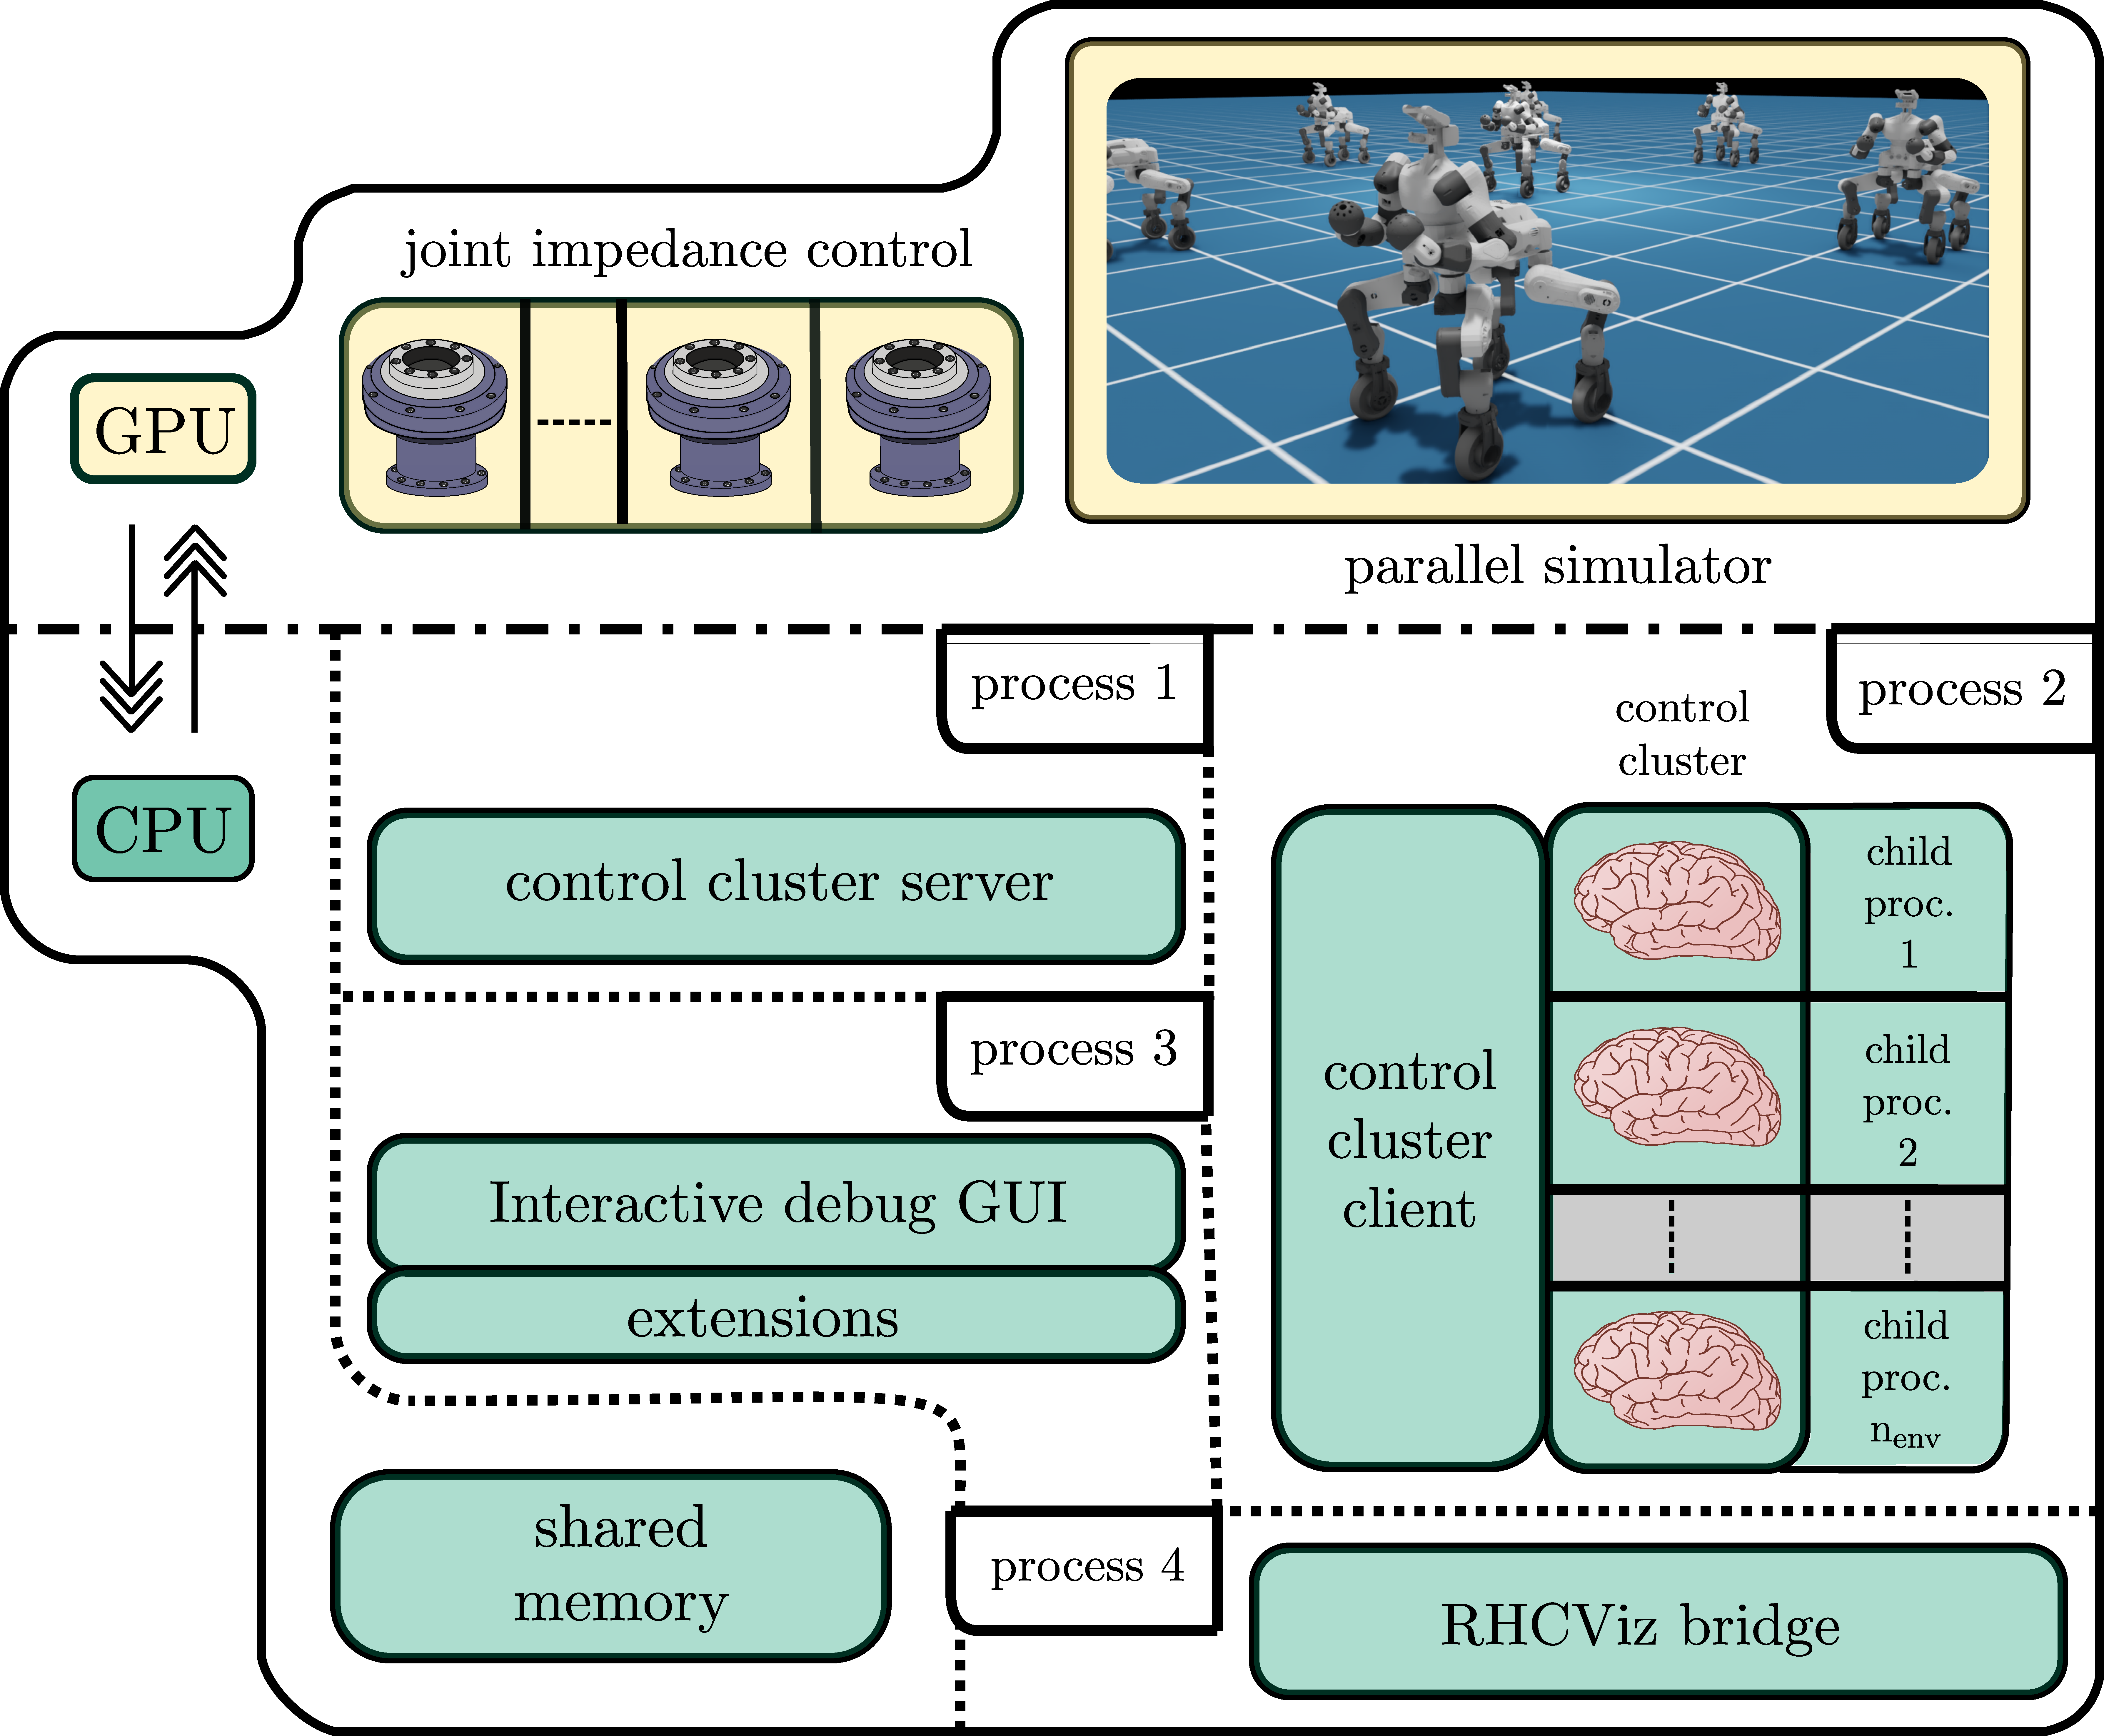
\includegraphics[width=0.9\columnwidth]{imgs/cocluster_arch.pdf}
	\caption{High-level overview of the software implementation of the training environment to which the agent is exposed: the robot in the simulator is controlled through a joint-level impedance controller, which is in turn used by a higher-level receding horizon controller. The agent can indirectly control the robot through the latter.}
	\label{fig:coclbridge_arch}
\end{figure}
\cite{rl:mujocoaccelereted2023}
\cite{frameworks:mittal2023orbit}

Fig.~\ref{fig:coclbridge_arch} shown a high level overview if the main moduli the echosystem is composed of. Specifically, it makes use of the following software packages:
\begin{itemize}
	\item Omniverse \textit{IsaacSim}~\cite{rl:makoviychuk2021isaac} is employed for performing the parallel GPU-accelerated simulation.
	\item \textit{Horizon}~\cite{frameworks::horizon_to} is employed for formulating the RHC controller, with an iLQR solver employed for computing the actual solution. Each controller is spawned in its own process using python's multiprocessing module.
	\item \textit{SharsorIPCpp}~\cite{mystuff::sharsoripcpp} is employed as a shared memory backend for fast data sharing between all the components on CPU.
	\item \textit{OmniRoboGym}~\cite{mystuff::omnirobogym} is used as a wrapper around IsaacSim and provides the \textit{simulation} environment.
	\item \textit{CoClusterBridge}~\cite{mystuff::coclusterbridge} is in charge of handling the connection and synchronization between the simulation environment and a cluster of RHC controllers. It furthermore provides an extensible debug GUI for monitoring the cluster and abstractions for the controllers.
	\item \textit{RHCViz}~\cite{mystuff::rhcviz} is a debug tool based on ROS1/ROS2 and RViz for visualizing RHC solutions in real-time. For our specific use case, it also allows to inspect a single environment during training without the need of any rendering on the simulator side.
	\item \textit{LRHControl}~\cite{mystuff::lrhccontrol} is the main package of the echosystem and is responsible for setting up the simulation environment, the control cluster, the (remote) training environment, the debug GUI (extensions included) and it currently utilizes a custom implementation of PPO~\cite{rl:schulman2017proximal} for training agents.
\end{itemize}




